\subsection{Детектирование слабого сигнала с помощью осциллятора Дуффинга}
\label{ssec:duffing}

Детектирование сигналов с расширенным спекторм (в частности сигналов системы Navstar GPS) с помощью осциллятора Дуффинга
достаточно новое направление в исследованиях по данной тематике. В частности
\cite{chaos_chen, chaos_cambridge, chaos_huang, chaos_song}. Так же является интересной более ранняя статья не рассматривающая GPS
\cite{chaos_wang}.

Осциллятор Дуффинга с периодическим внешним воздействием может быть описан уравнением \ref{eq:duffing}:

\begin{center}
\begin{equation}
	\label{eq:duffing}
	mx'' + cx' + k_{1}x + k_{2}x^3 = F_{0}\cos(\omega{t})
\end{equation}
\end{center}

где
$m$- масса,
$c$ - коэффициент диссипации,
$x$ - состояние осциллятора,
$k_1$ и $k_2$ - линейный и нелинейный коэффициенты соответственно.
$F_{0}\cos(\omega{t})$ - внешнее воздействие.

Подробно уравнение \ref{eq:duffing} рассмотрено в \cite{chaos_neimark_landa} (Глава 9 параграф 3). Но
для использования осциллятора Дуффинга для детектирования сигналов системы GPS былa предложена
усовершенствованная форма данного осциллятора \cite{chaos_song, chaos_chen}:

\begin{center}
\begin{equation}
	\label{eq:duffing_gps}
	x'' +cx' - x^3 + x^5 = \gamma\cos(\omega{t}) + (\gamma_{x}\cos(\omega_{x}) + n(t))
\end{equation}
\end{center}

Перепишем динамическую систему \ref{eq:duffing_gps} в виде:
\begin{center}
\begin{eqnarray}
	\label{eq:duffing_gps_2}
	y(t) & = & x'(t) \\
	y'(t) & = & -cx' + x^3 - x^5 + \gamma\cos(\omega{t}) + (\gamma_{x}\cos(\omega_{x}) + n(t))
\end{eqnarray}
\end{center}

Пример фазового портрета при ${\omega=\omega_{x}}$ изображен на рисунке \ref{pic:duffing_sync},
фазовый портрет хаоса расположен на рисунках \ref{pic:duffing_chaos1}, \ref{pic:duffing_chaos2}

\begin{figure}[H]
	\center\scalebox{0.5}{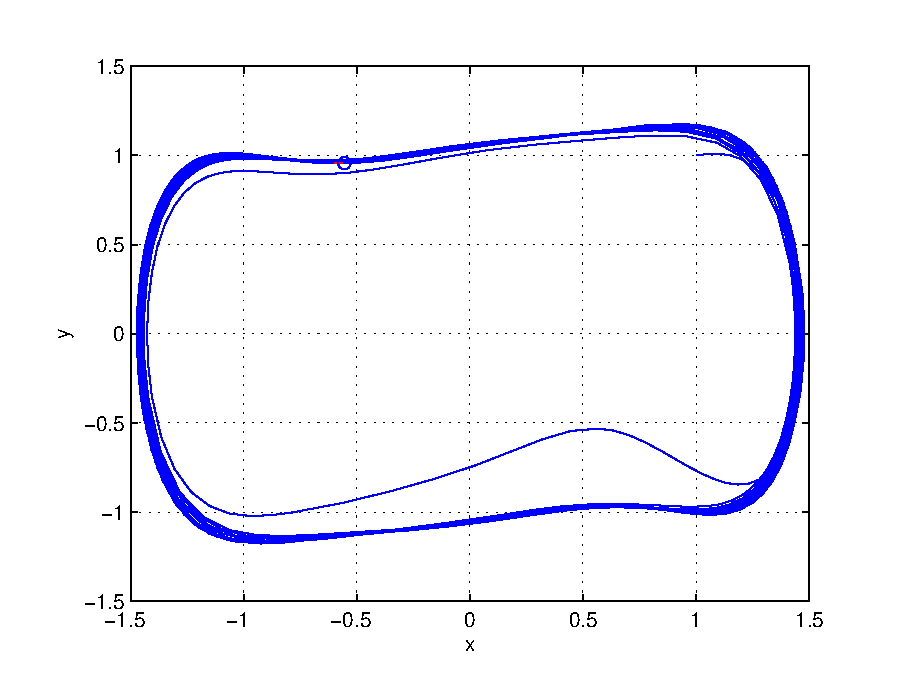
\includegraphics[width=1\linewidth]{duffing_sync.eps}}
	\caption{Фазовый портрет при ${\omega =\omega_{x}}$}
	\label{pic:duffing_sync}
\end{figure}

\begin{figure}[H]
	\center\scalebox{0.5}{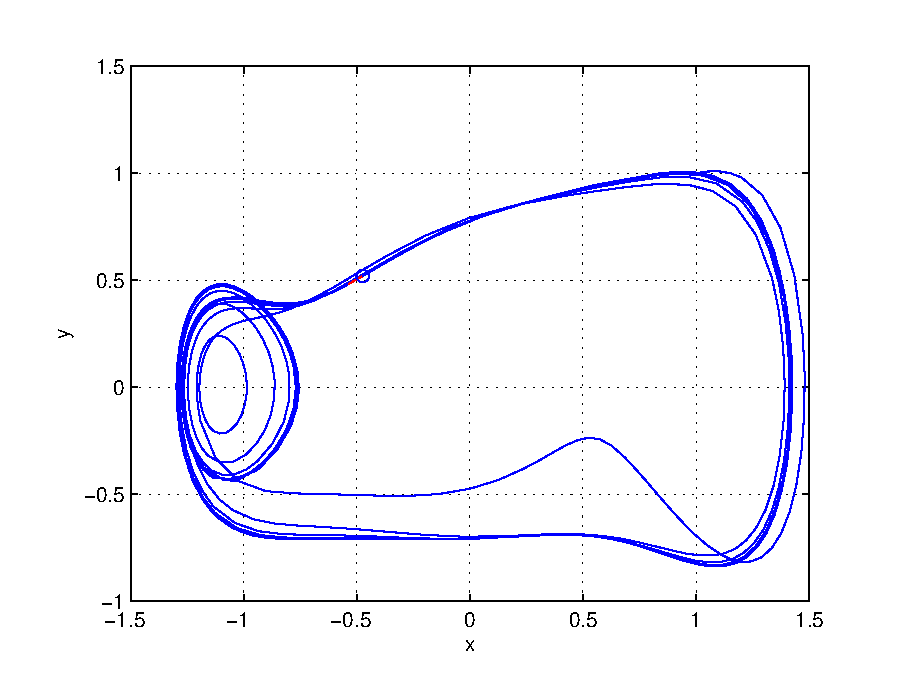
\includegraphics[width=1\linewidth]{duffing_chaos1.eps}}
	\caption{Фазовый портрет при ${\omega < \omega_{x}}$}
	\label{pic:duffing_chaos1}
\end{figure}

\begin{figure}[H]
	\center\scalebox{0.5}{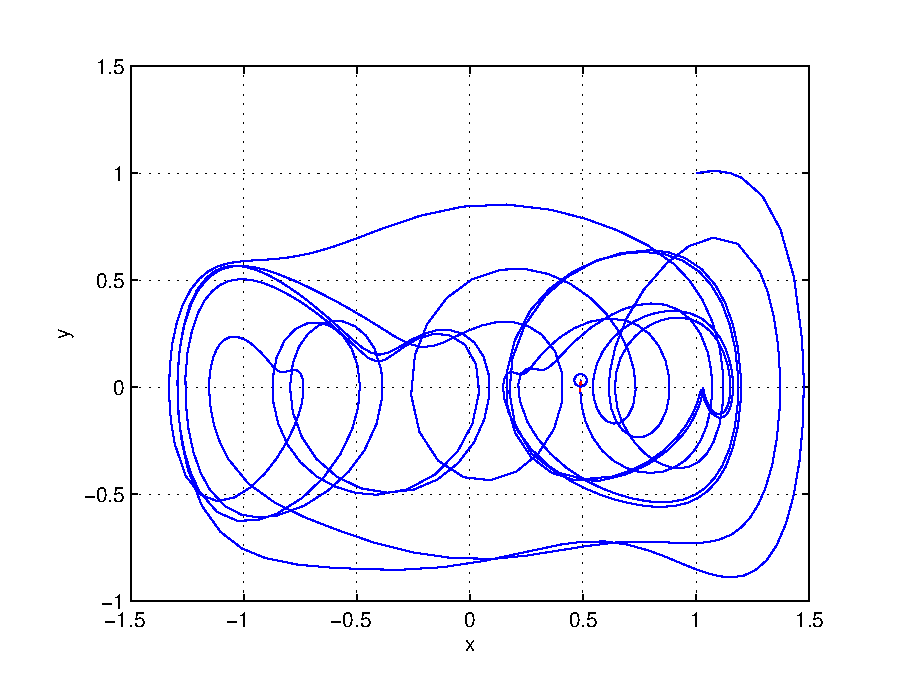
\includegraphics[width=1\linewidth]{duffing_chaos2.eps}}
	\caption{Фазовый портрет при ${\omega > \omega_{x}}$}
	\label{pic:duffing_chaos2}
\end{figure}

В качестве параметров уравнения применялись $c = 0.5$, $\gamma=\gamma_{x}=0.36$, ${\omega=1}$

Часто для вычисления характеристик хаотической динамики применяется экспонента Ляпунова.
Она описывает метод определения в каком состоянии находится система. Если система находится
в стабильном состоянии линии фазовой траектории будут близко прилегать одна к другой, в противном
случае система находится в состоянии хаоса.

В статье \cite{chaos_chen} предложен усовершенствованный метод, базирующийся на вычислении дисперсии
фазовой траектории. Действительно, на рисунках \ref{pic:duffing_sync}, \ref{pic:duffing_chaos1},
\ref{pic:duffing_chaos2} видно - когда система находится в хаотическом состоянии значение
дисперсии ниже, чем соответствующее значение в состоянии $\omega = \omega_{x}$. На основе этого была
предложена усовершенствованная схема детектора сигнала \ref{pic:chaos_acq}


\newpage
